\documentclass[journal,12pt,twocolumn]{IEEEtran}

\usepackage{setspace}
\usepackage{gensymb}

\singlespacing


\usepackage[cmex10]{amsmath}

\usepackage{amsthm}

\usepackage{mathrsfs}
\usepackage{txfonts}
\usepackage{stfloats}
\usepackage{bm}
\usepackage{cite}
\usepackage{cases}
\usepackage{subfig}

\usepackage{longtable}
\usepackage{multirow}

\usepackage{enumitem}
\usepackage{mathtools}
\usepackage{steinmetz}
\usepackage{tikz}
\usepackage{circuitikz}
\usepackage{verbatim}
\usepackage{tfrupee}
\usepackage[breaklinks=true]{hyperref}
\usepackage{graphicx}
\usepackage{tkz-euclide}
\usepackage{float}

\usetikzlibrary{calc,math}
\usepackage{listings}
    \usepackage{color}                                            %%
    \usepackage{array}                                            %%
    \usepackage{longtable}                                        %%
    \usepackage{calc}                                             %%
    \usepackage{multirow}                                         %%
    \usepackage{hhline}                                           %%
    \usepackage{ifthen}                                           %%
    \usepackage{lscape}     
\usepackage{multicol}
\usepackage{chngcntr}

\DeclareMathOperator*{\Res}{Res}

\renewcommand\thesection{\arabic{section}}
\renewcommand\thesubsection{\thesection.\arabic{subsection}}
\renewcommand\thesubsubsection{\thesubsection.\arabic{subsubsection}}

\renewcommand\thesectiondis{\arabic{section}}
\renewcommand\thesubsectiondis{\thesectiondis.\arabic{subsection}}
\renewcommand\thesubsubsectiondis{\thesubsectiondis.\arabic{subsubsection}}


\hyphenation{op-tical net-works semi-conduc-tor}
\def\inputGnumericTable{}                                 %%

\lstset{
%language=C,
frame=single, 
breaklines=true,
columns=fullflexible
}
\begin{document}


\newtheorem{theorem}{Theorem}[section]
\newtheorem{problem}{Problem}
\newtheorem{proposition}{Proposition}[section]
\newtheorem{lemma}{Lemma}[section]
\newtheorem{corollary}[theorem]{Corollary}
\newtheorem{example}{Example}[section]
\newtheorem{definition}[problem]{Definition}

\newcommand{\BEQA}{\begin{eqnarray}}
\newcommand{\EEQA}{\end{eqnarray}}
\newcommand{\define}{\stackrel{\triangle}{=}}
\bibliographystyle{IEEEtran}
\providecommand{\mbf}{\mathbf}
\providecommand{\pr}[1]{\ensuremath{\Pr\left(#1\right)}}
\providecommand{\qfunc}[1]{\ensuremath{Q\left(#1\right)}}
\providecommand{\sbrak}[1]{\ensuremath{{}\left[#1\right]}}
\providecommand{\lsbrak}[1]{\ensuremath{{}\left[#1\right.}}
\providecommand{\rsbrak}[1]{\ensuremath{{}\left.#1\right]}}
\providecommand{\brak}[1]{\ensuremath{\left(#1\right)}}
\providecommand{\lbrak}[1]{\ensuremath{\left(#1\right.}}
\providecommand{\rbrak}[1]{\ensuremath{\left.#1\right)}}
\providecommand{\cbrak}[1]{\ensuremath{\left\{#1\right\}}}
\providecommand{\lcbrak}[1]{\ensuremath{\left\{#1\right.}}
\providecommand{\rcbrak}[1]{\ensuremath{\left.#1\right\}}}
\theoremstyle{remark}
\newtheorem{rem}{Remark}
\newcommand{\sgn}{\mathop{\mathrm{sgn}}}
\providecommand{\abs}[1]{\left\vert#1\right\vert}
\providecommand{\res}[1]{\Res\displaylimits_{#1}} 
\providecommand{\norm}[1]{\left\lVert#1\right\rVert}
%\providecommand{\norm}[1]{\lVert#1\rVert}
\providecommand{\mtx}[1]{\mathbf{#1}}
\providecommand{\mean}[1]{E\left[ #1 \right]}
\providecommand{\fourier}{\overset{\mathcal{F}}{ \rightleftharpoons}}
%\providecommand{\hilbert}{\overset{\mathcal{H}}{ \rightleftharpoons}}
\providecommand{\system}{\overset{\mathcal{H}}{ \longleftrightarrow}}
	%\newcommand{\solution}[2]{\textbf{Solution:}{#1}}
\newcommand{\solution}{\noindent \textbf{Solution: }}
\newcommand{\cosec}{\,\text{cosec}\,}
\providecommand{\dec}[2]{\ensuremath{\overset{#1}{\underset{#2}{\gtrless}}}}
\newcommand{\myvec}[1]{\ensuremath{\begin{pmatrix}#1\end{pmatrix}}}
\newcommand{\mydet}[1]{\ensuremath{\begin{vmatrix}#1\end{vmatrix}}}
\numberwithin{equation}{subsection}
\makeatletter
\@addtoreset{figure}{problem}
\makeatother
\let\StandardTheFigure\thefigure
\let\vec\mathbf
\renewcommand{\thefigure}{\theproblem}
\def\putbox#1#2#3{\makebox[0in][l]{\makebox[#1][l]{}\raisebox{\baselineskip}[0in][0in]{\raisebox{#2}[0in][0in]{#3}}}}
     \def\rightbox#1{\makebox[0in][r]{#1}}
     \def\centbox#1{\makebox[0in]{#1}}
     \def\topbox#1{\raisebox{-\baselineskip}[0in][0in]{#1}}
     \def\midbox#1{\raisebox{-0.5\baselineskip}[0in][0in]{#1}}
\vspace{3cm}
\title{Challenge Problem 3}
\author{K.A. Raja Babu}
\maketitle
\newpage
\bigskip
\renewcommand{\thefigure}{\theenumi}
\renewcommand{\thetable}{\theenumi}
Download all python codes from 
\begin{lstlisting}
https://github.com/ka-raja-babu/Matrix-Theory/tree/main/ChallengeProblem3/Codes
\end{lstlisting}
%
and latex-tikz codes from 
%
\begin{lstlisting}
https://github.com/ka-raja-babu/Matrix-Theory/tree/main/ChallengeProblem3
\end{lstlisting}
%
\section{Challenge Question 3}

For the quadratic equation to not have any real roots, the y coordinate should always be either positive or negative . Express this in terms of the matrix/vector parameters of the parabola .

\section{Solution}

The general form of a quadratic equation is 
\begin{align}
    y = ax^2+bx+c \\
    \implies ax^2+bx+c-y = 0
\end{align}

which can be written in vector form as
\begin{align}
    \vec{x}^T\vec{V}\vec{x} + 2\vec{u}^T\vec{x} + f &= 0
\end{align}

where
\begin{align}
    \vec{V} &= \myvec{a & 0 \\ 0 & 0}
    \\
    \vec{u} &= \myvec{\frac{b}{2} \\ \frac{-1}{2}}
    \\
    f &= c
\end{align}

Using eigenvalue decomposition,
\begin{align}
    \vec{D} &= \myvec{0 & 0 \\ 0 & a} \\
    \vec{P} &= \myvec{0 & 1 \\ 1 & 0}
\end{align}

Also,
\begin{align}
    \eta &= \vec{u}^T\vec{p_1}
    \\
    &= \frac{-1}{2}
\end{align}

Now,for y coordinate to be always positive,two conditions need to be satisfied:
\begin{enumerate}
 \item y-coordinate of vertex $\vec{c}$ of parabola needs to be always positive.
 \item Coefficient $a$ of $x^2$ needs to be always positive.
\end{enumerate}

$\therefore$ For condition 1:
\begin{align}
    \myvec{\vec{u}^T + \eta\vec{p_1}^T \\ \vec{V}}\vec{c} &= \myvec{-f \\ \eta\vec{p_1}-\vec{u}} \\
    \vec{p_1}^T\vec{c} &> 0
\end{align}

For condition 2:
\begin{align}
    \vec{p_2}^T\vec{V}\vec{p_2} > 0
\end{align}

And,for y coordinate to be always negative,two conditions need to be satisfied:
\begin{enumerate}
 \item y-coordinate of vertex $\vec{c}$ of parabola needs to be always negative.
 \item Coefficient $a$ of $x^2$ needs to be always negative.
\end{enumerate}

$\therefore$ For condition 1:
\begin{align}
    \myvec{\vec{u}^T + \eta\vec{p_1}^T \\ -\vec{V}}\vec{c} &= \myvec{-f \\ \eta\vec{p_1}-\vec{u}} \\
    \vec{p_1}^T\vec{c} &< 0
\end{align}

For condition 2:
\begin{align}
    \vec{p_2}^T\vec{V}\vec{p_2} < 0
\end{align}

Hence,condition for non-real roots in terms of matrix/vector parameters of the parabola is 
\begin{align}
    \boxed{(\vec{p_1}^T\vec{c})(\vec{p_2}^T\vec{V}\vec{p_2}) > 0}
\end{align}

\section{Examples}
\begin{enumerate}
    \item 
    \begin{align}
        y &= 21x^2-28x+10
    \end{align}
    Here,
    \begin{align}
        \vec{V} = \myvec{21 & 0 \\ 0 & 0},\vec{u}=-\myvec{14 \\ \frac{1}{2}},f=10
    \end{align}
    Using eigenvalue decomposition,
    \begin{align}
        \vec{D} = \myvec{0 & 0\\0 & 21} ,\vec{P}=\myvec{0 & 1\\1 & 0}
    \end{align}
    $\therefore$Vertex $\vec{c}$ is given by
    \begin{align}
        \myvec{-14 & -1 \\ 21 & 0 \\ 0 & 0}\vec{c} &= \myvec{-10 \\ 14 \\ 0} \\
        \implies  \myvec{-14 & -1 \\ 21 & 0}\vec{c} &= \myvec{-10 \\ 14}
        \\
        \implies \vec{c} &= \myvec{\frac{2}{3} \\ \frac{2}{3}}
    \end{align}
    Now,
    \begin{align}
        \vec{p_1}^T\vec{c} &= \myvec{0 & 1}\myvec{\frac{2}{3} \\ \frac{2}{3}}
        \\
        &= \frac{2}{3}
    \end{align}
    and,
    \begin{align}
        \vec{p_2}^T\vec{V}\vec{p_2} &= \myvec{1 & 0}\myvec{21 & 0\\0& 0}\myvec{1 \\ 0}
        \\
        &= 21
    \end{align}
    $\because$
    \begin{align}
    (\vec{p_1}^T\vec{c})(\vec{p_2}^T\vec{V}\vec{p_2}) = (\frac{2}{3})(21) = \frac{42}{3}>0
    \end{align}
    Hence,the given equation does not have any real roots.
    
    \numberwithin{figure}{section}
    \begin{figure}[!ht]
    \centering
    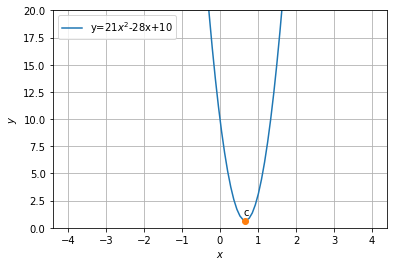
\includegraphics[width=\columnwidth]{ChallengeProblem3_2.png}
    \caption{$y=21x^2-28x+10$}
    \label{ex1}	
    \end{figure}
    
    \item
    \begin{align}
        y &= 6x^2-x-2
    \end{align}
    Here,
    \begin{align}
        \vec{V} = \myvec{6 & 0 \\ 0 & 0},\vec{u}=-\myvec{\frac{1}{2} \\ \frac{1}{2}},f=-2
    \end{align}
    Using eigenvalue decomposition,
    \begin{align}
        \vec{D} = \myvec{0 & 0\\0 & 6} ,\vec{P}=\myvec{0 & 1\\1 & 0}
    \end{align}
    $\therefore$Vertex $\vec{c}$ is given by
    \begin{align}
        \myvec{\frac{-1}{2} & -1 \\ 6 & 0 \\ 0 & 0}\vec{c} &= \myvec{2 \\ \frac{1}{2} \\ 0} \\
        \implies  \myvec{\frac{-1}{2} & -1 \\ 6 & 0}\vec{c} &= \myvec{2 \\ \frac{1}{2}}
        \\
        \implies \vec{c} &= \myvec{\frac{1}{12} \\ \frac{-49}{24}}
    \end{align}
    Now,
    \begin{align}
        \vec{p_1}^T\vec{c} &= \myvec{0 & 1}\myvec{\frac{1}{12} \\ \frac{-49}{24}}
        \\
        &= \frac{-49}{24}
    \end{align}
    and,
    \begin{align}
        \vec{p_2}^T\vec{V}\vec{p_2} &= \myvec{1 & 0}\myvec{6 & 0\\0& 0}\myvec{1 \\ 0}
        \\
        &= 6
    \end{align}
    $\because$
    \begin{align}
    (\vec{p_1}^T\vec{c})(\vec{p_2}^T\vec{V}\vec{p_2}) = (\frac{-49}{24})(6) = \frac{-49}{4}<0
    \end{align}
    Hence,the given equation has real roots.
    
    \numberwithin{figure}{section}
    \begin{figure}[!ht]
    \centering
    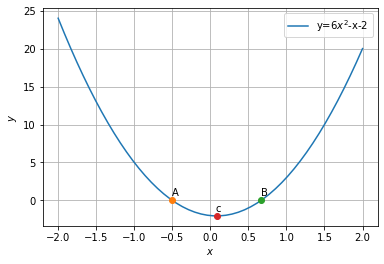
\includegraphics[width=\columnwidth]{ChallengeProblem3_1.png}
    \caption{$y=6x^2-x-2$}
    \label{ex2}	
    \end{figure}
    
    \item
    \begin{align}
        y &= -x^2-4x-5
    \end{align}
    Here,
    \begin{align}
        \vec{V} = \myvec{-1 & 0 \\ 0 & 0},\vec{u}=-\myvec{2 \\ \frac{1}{2}},f=-5
    \end{align}
    
    Using eigenvalue decomposition,
    \begin{align}
        \vec{D} = \myvec{0 & 0\\0 & -1} ,\vec{P}=\myvec{0 & 1\\1 & 0}
    \end{align}
    $\therefore$Vertex $\vec{c}$ is given by
    \begin{align}
        \myvec{-2 & -1 \\ 1 & 0 \\ 0 & 0}\vec{c} &= \myvec{5 \\ 2 \\ 0} \\
        \implies  \myvec{-2 & -1 \\ 1 & 0}\vec{c} &= \myvec{5 \\ 2}
        \\
        \implies \vec{c} &= \myvec{2\\-1}
    \end{align}
    
    Now,
    \begin{align}
        \vec{p_1}^T\vec{c} &= \myvec{0 & 1}\myvec{2 \\ -1}
        \\
        &= -1
    \end{align}
    and,
    \begin{align}
        \vec{p_2}^T\vec{V}\vec{p_2} &= \myvec{1 & 0}\myvec{-1 & 0\\0& 0}\myvec{1 \\ 0}
        \\
        &= -1
    \end{align}
    
    \numberwithin{figure}{section}
    \begin{figure}[!ht]
    \centering
    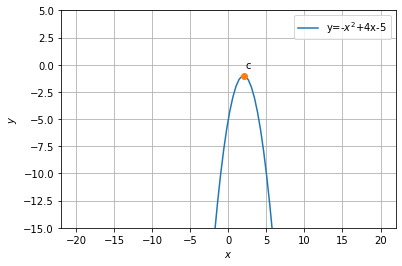
\includegraphics[width=\columnwidth]{ChallengeProblem3_3.png}
    \caption{$y=-x^2+4x-5$}
    \label{ex4}	
    \end{figure}
    
    $\because$
    \begin{align}
    (\vec{p_1}^T\vec{c})(\vec{p_2}^T\vec{V}\vec{p_2}) = (-1)(-1) = 1>0
    \end{align}
    Hence,the given equation does not have real roots.
  
    \item
    \begin{align}
        y &= -x^2-4x+9
    \end{align}
    Here,
    \begin{align}
        \vec{V} = \myvec{-1 & 0 \\ 0 & 0},\vec{u}=-\myvec{2 \\ \frac{1}{2}},f=9
    \end{align}
  
    Using eigenvalue decomposition,
    \begin{align}
        \vec{D} = \myvec{0 & 0\\0 & -1} ,\vec{P}=\myvec{0 & 1\\1 & 0}
    \end{align}
    $\therefore$Vertex $\vec{c}$ is given by
    \begin{align}
        \myvec{-2 & -1 \\ 1 & 0 \\ 0 & 0}\vec{c} &= \myvec{-9 \\ 2 \\ 0} \\
        \implies  \myvec{-2 & -1 \\ 1 & 0}\vec{c} &= \myvec{-9 \\ 2}
        \\
        \implies \vec{c} &= \myvec{2\\13}
    \end{align}
    
    \numberwithin{figure}{section}
    \begin{figure}[!ht]
    \centering
    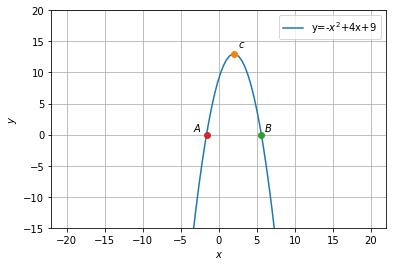
\includegraphics[width=\columnwidth]{ChallengeProblem3_4.png}
    \caption{$y=-x^2+4x+9$}
    \label{ex3}	
    \end{figure}
    
    Now,
    \begin{align}
        \vec{p_1}^T\vec{c} &= \myvec{0 & 1}\myvec{2 \\ 13}
        \\
        &= 13
    \end{align}
    and,
    \begin{align}
        \vec{p_2}^T\vec{V}\vec{p_2} &= \myvec{1 & 0}\myvec{-1 & 0\\0& 0}\myvec{1 \\ 0}
        \\
        &= -1
    \end{align}
    $\because$
    \begin{align}
    (\vec{p_1}^T\vec{c})(\vec{p_2}^T\vec{V}\vec{p_2}) = (13)(-1) = -13<0
    \end{align}
    Hence,the given equation has real roots.
\end{enumerate}

\end{document}